% --------------------------------------------------------------------------------

\begin{exercise}[Exercise 3.22]

Consider the continuing MDP shown below.
The only decision to be made is that in the top state, where two actions are available, \textbf{left} and \textbf{right}.
The numbers show the rewards that are received deterministically after each action.
There are exactly two deterministic policies, $\pi_\textbf{left}$ and $\pi_\textbf{right}$.
What policy is optimal if $\gamma = 0$?
If $\gamma = 0.9$?
If $\gamma = 0.5$?

\begin{figure}[H]
    \centering
    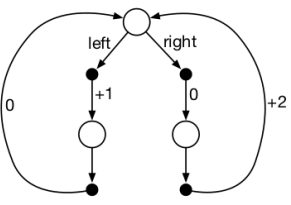
\includegraphics[width = 0.25 \textwidth]{2.20.png}
    \caption{}
    \label{fig:2.20}
\end{figure}

\end{exercise}

% --------------------------------------------------------------------------------

\begin{solution}

When using the policies $\pi_\textbf{left}$ or $\pi_\textbf{right}$ we always chose the corresponding action with certainty $1$.

\begin{align*}
    v_\pi(s)
    & =
    \E_\pi
    \bbraces
    {
        \sum_{k=0}^\infty
            \gamma^k R_{t+k+1}
        \mid
        S_t = s
    } \\
    & =
    \sum_{k=0}^\infty
        \gamma^k
        \E_\pi[R_{t+k+1} \mid S_t = s] \\
    & =
    \E_\pi[R_{t+1} \mid S_t = s]
    +
    \sum_{k \in 2 \N + 2}
        \gamma^k
        \E_\pi[R_{t+k+1} \mid S_t = s]
    +
    \sum_{k \in 2 \N + 1}
        \gamma^k
        \E_\pi[R_{t+k+1} \mid S_t = s] \\
    & =
    \begin{cases}
        \sum_{k=0}^\infty \gamma^{2 k} = \frac{1}{1 - \gamma^2},
        & \pi = \pi_\textbf{left},  \quad s = \textbf{upper}, \\
        2 \sum_{k=0}^\infty \gamma^{2 k + 1} = \frac{2 \gamma}{1 - \gamma^2},
        & \pi = \pi_\textbf{right}, \quad s = \textbf{upper}, \\
        \sum_{k=0}^\infty \gamma^{2 k  + 1} = \frac{\gamma}{1 - \gamma^2},
        & \pi = \pi_\textbf{left},  \quad s = \textbf{left},  \\
        2 \sum_{k=0}^\infty \gamma^{2 k + 2} = \frac{2 \gamma^2}{1 - \gamma^2},
        & \pi = \pi_\textbf{right}, \quad s = \textbf{left},  \\
        2 + \sum_{k=0}^\infty \gamma^{2 k + 2} = 2 + \frac{2 \gamma^2}{1 - \gamma^2} = \frac{2}{1 - \gamma^2},
        & \pi = \pi_\textbf{left},  \quad s = \textbf{right}, \\
        2 \sum_{k=0}^\infty \gamma^{2 k} = \frac{2}{1 - \gamma^2},
        & \pi = \pi_\textbf{right}, \quad s = \textbf{right}
    \end{cases}
\end{align*}

\begin{align*}
    \begin{array}{c|c|c|c}
        \gamma & \pi                & s              & v_\pi(s)           \\ \hline
        0      & \pi_\textbf{left}  & \textbf{upper} & 1                  \\
        0      & \pi_\textbf{right} & \textbf{upper} & 0                  \\
        0      & \pi_\textbf{left}  & \textbf{left}  & 0                  \\
        0      & \pi_\textbf{right} & \textbf{left}  & 0                  \\
        0      & \pi_\textbf{left}  & \textbf{right} & 2                  \\
        0      & \pi_\textbf{right} & \textbf{right} & 2                  \\
        0.9    & \pi_\textbf{left}  & \textbf{upper} & \nicefrac{100}{19} \\
        0.9    & \pi_\textbf{right} & \textbf{upper} & \nicefrac{180}{19} \\
        0.9    & \pi_\textbf{left}  & \textbf{left}  & \nicefrac{90} {19} \\
        0.9    & \pi_\textbf{right} & \textbf{left}  & \nicefrac{162}{19} \\
        0.9    & \pi_\textbf{left}  & \textbf{right} & \nicefrac{200}{19} \\
        0.9    & \pi_\textbf{right} & \textbf{right} & \nicefrac{200}{19} \\
        0.5    & \pi_\textbf{left}  & \textbf{upper} & \nicefrac{4}{3}    \\
        0.5    & \pi_\textbf{right} & \textbf{upper} & \nicefrac{4}{3}    \\
        0.5    & \pi_\textbf{left}  & \textbf{left}  & \nicefrac{2}{3}    \\
        0.5    & \pi_\textbf{right} & \textbf{left}  & \nicefrac{2}{3}    \\
        0.5    & \pi_\textbf{left}  & \textbf{right} & \nicefrac{8}{3}    \\
        0.5    & \pi_\textbf{right} & \textbf{right} & \nicefrac{8}{3}    \\
    \end{array}
\end{align*}

\begin{align*}
    \begin{array}{c|c}
        \gamma & \pi_\ast                           \\ \hline
        0   & \pi_\textbf{left}                     \\
        0.9 & \pi_\textbf{right}                    \\
        0.5 & \pi_\textbf{left}, \pi_\textbf{right} \\
    \end{array}
\end{align*}

\end{solution}

% --------------------------------------------------------------------------------
